\documentclass[spanish,12pt,a4paper,titlepage]{report}
\usepackage[utf8]{inputenc}
\usepackage{graphicx}
\usepackage{subfig}
\usepackage{float}
\usepackage{wrapfig}
\usepackage{multirow}
\usepackage{caption}
\usepackage[spanish]{babel}
\usepackage[dvips]{hyperref}
\usepackage{amssymb}
\usepackage{listings}
\usepackage{epsfig}
\usepackage{amsmath}
\usepackage{array}
\usepackage[table]{xcolor}
\usepackage{multirow}
%\usepackage[Sonny]{fncychap}
\usepackage[Lenny]{fncychap}
%\usepackage[Glenn]{fncychap}
%\usepackage[Conny]{fncychap}
%\usepackage[Rejne]{fncychap}
%\usepackage[Bjarne]{fncychap}
%\usepackage[Bjornstrup]{fncychap}

%\usepackage{subfiles}
%\usepackage{framed}

\setlength{\topmargin}{-1.5cm}
\setlength{\textheight}{25cm}
\setlength{\oddsidemargin}{0.3cm} 
\setlength{\textwidth}{15cm}
\setlength{\columnsep}{0cm}



\newcommand{\HRule}{\rule{\linewidth}{0.5mm}}
\begin{document}

% ------------------------------------------------------------------ %
% -----------------------  Empieza el Título ----------------------- %
% ------------------------------------------------------------------ %
\begin{titlepage}
\begin{center}
\HRule \\[0.4cm]
{ \huge \bfseries La mujer más hermosa del mundo}\\[0.4cm]
\HRule \\[2.5cm]
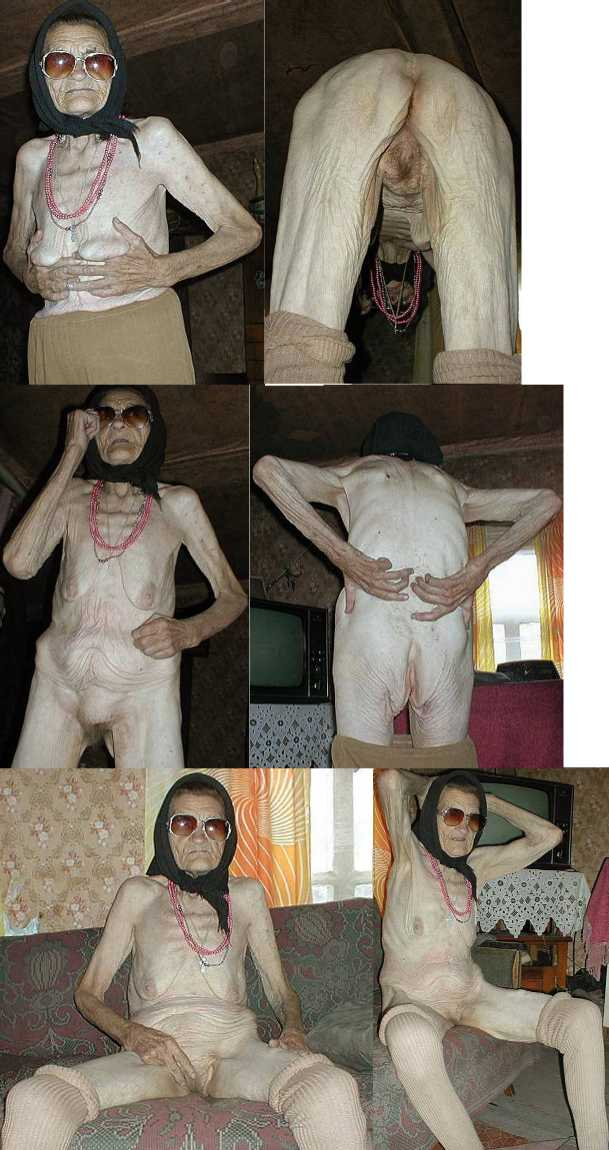
\includegraphics[width=.7\textwidth]{./pics/19.jpg}\\[1cm]
\vfill
\end{center}
\end{titlepage}
% ------------------------------------------------------------------ %
% -----------------------  Termina el Título ----------------------- %
% ------------------------------------------------------------------ %

\chapter{Calibración de giróscopo}

\section{Objetivos}

\begin{itemize}
	\item Realizar una serie de pruebas con el fin de calibrar el giróscopo de tres ejes de la IMU.
	\item Estudiar, proponer y validar un modelo posible para dicha calibración.
	\item Estimar las fuentes de error del mismo (ruido y bias).
\end{itemize}

\section{Materiales}
\begin{itemize}
\item Mongoose 9Dof IMU de \emph{Ckdevices}
\item Beagleboard xM
\item Adaptador Wi-Fi 
\item Tocadiscos
\item Cronómetro
\item Cubo perfecto de madera
\item 2 escuadras de 45º
\item 2 escuadras de 30º
\item Madera de 4 cm de ancho con lados paralelos
\end{itemize}

\section{Marco teórico}
Para la calibración del giróscopo se utiliza el mismo modelo que se utilizó para el acelerómetro en la sección \ref{chap:calibracion_acelerometro}, se estudia las no idealidades que afectan la lectura de los valores de velocidad angular registrados en el dispositivo y se validan los resultados obtenidos. Las no idealidades  a considerar basados en lo desarrollado por \cite{bib:calib_IMU} son:

\begin{itemize}
\item Ruido inherente
\item Relación entre aceleración real y lectura del acelerómetro no lineal.
\item No ortogonalidad de los ejes
\item Drift aleatorio
\item Variación de las medidas con la temperatura
\end{itemize}

El modelo para la calibración del giróscopo, como puede verse con más detalle en el capítulo \ref{chap:calibracion_acelerometro}, es:
$$\tilde{\mathbf{w^a}}=K_w(T_a^p)^{-1}\mathbf{w^p}+b_w$$
con $K_w$ matriz diagonal que representa el factor de escala para convertir del valor digital a la aceleración correspondiente, $\mathbf{b}_w$ un término independiente para corregir la posición del cero y $T^p_a$ una matriz que corrige la no perpendicularidad perfecta de los ejes:
$$T^p_a=\left( 
\begin{matrix}
1 &-\alpha_{yz} &\alpha_{zy}\\
\alpha_{xz} &1& -\alpha_{zx} \\
-\alpha_{xy} &\alpha_{yx} &1\\
\end{matrix} 
\right)$$

A su vez, estos parámetros varían con la temperatura, lo cual puede introducir errores significativos dependiendo del estado del tiempo, la estación del año, o la hora del día

\section{Procedimiento}
\subsection{Caracterización de las no idealidades variables}

Para obtener más información sobre el \emph{ruido inherente} y el \emph{drift aleatorio} se toman datos durante una hora a una frecuencia de 50 Hz con el dispositivo quieto.\\

\subsection{Determinación de parámetros estáticos}

Para poder realizar la calibración pertinente es necesario determinar 12 parámetros: las ganancias y bias de los 3 ejes y los 6 ángulos de la matriz $T^p_a$. Para determinar dichos parámetros es conveniente obtener el doble o triple de medidas que de parámetros. Las medidas a realizar son las siguientes:

\begin{table}[H]
\centering
\begin{small}
\begin{tabular}{|c|c|c|}
\hline
  {\cellcolor[gray]{0.85} \centering \textbf{Eje de giro principal}}
& {\cellcolor[gray]{0.85} \centering \textbf{Eje de giro secundario}}
& {\cellcolor[gray]{0.85} \centering \textbf{Ángulo de giro}} \\ \hline  \hline
x & z & 0 \\ \hline
x & z & 30 \\ \hline
x & z & 45 \\ \hline
y & x & 0 \\ \hline
y & x & 30 \\ \hline
y & x & 45 \\ \hline
z & y & 0 \\ \hline
z & y & 30 \\ \hline
z & y & 45 \\ \hline
\end{tabular}
\caption{Configuraciones utilizadas para calibrar el giróscopo}
\label{tab:gyros}
\end{small}
\end{table} 

Con un total de 9 configuraciones diferentes, donde cada una de ellas aporta 3 medidas (una por cada eje), se utilizarán un total de 27 medidas para determinar los 12 parámetros involucrados.

\subsubsection*{Preparación}

Las medidas consisten básicamente en dejar la IMU girar a la velocidad del tocadiscos en las posiciones listadas en la tabla \ref{tab:gyros}. La dirección de giro principal es la dirección de giro del tocadiscos cuando no hay giro en la dirección secundaria. Con el cubo de madera se resuelven las rotaciones de 90 grados para alinear los diferentes ejes de la IMU con el eje de giro del tocadiscos. Los giros en el eje secundario se realizan utilizando las escuadras y la madera de 4 cm de ancho y lados paralelos, como se muestra en la figura \ref{fig:escuadras}. Apoyando el cubo sobre la escuadra se logran los ángulos de $30º$ y $45º$ deseados en las direcciones de giro secundarias.

\begin{wrapfigure}{l}{0.6\textwidth}
  \vspace{-20pt}
  \begin{center}
    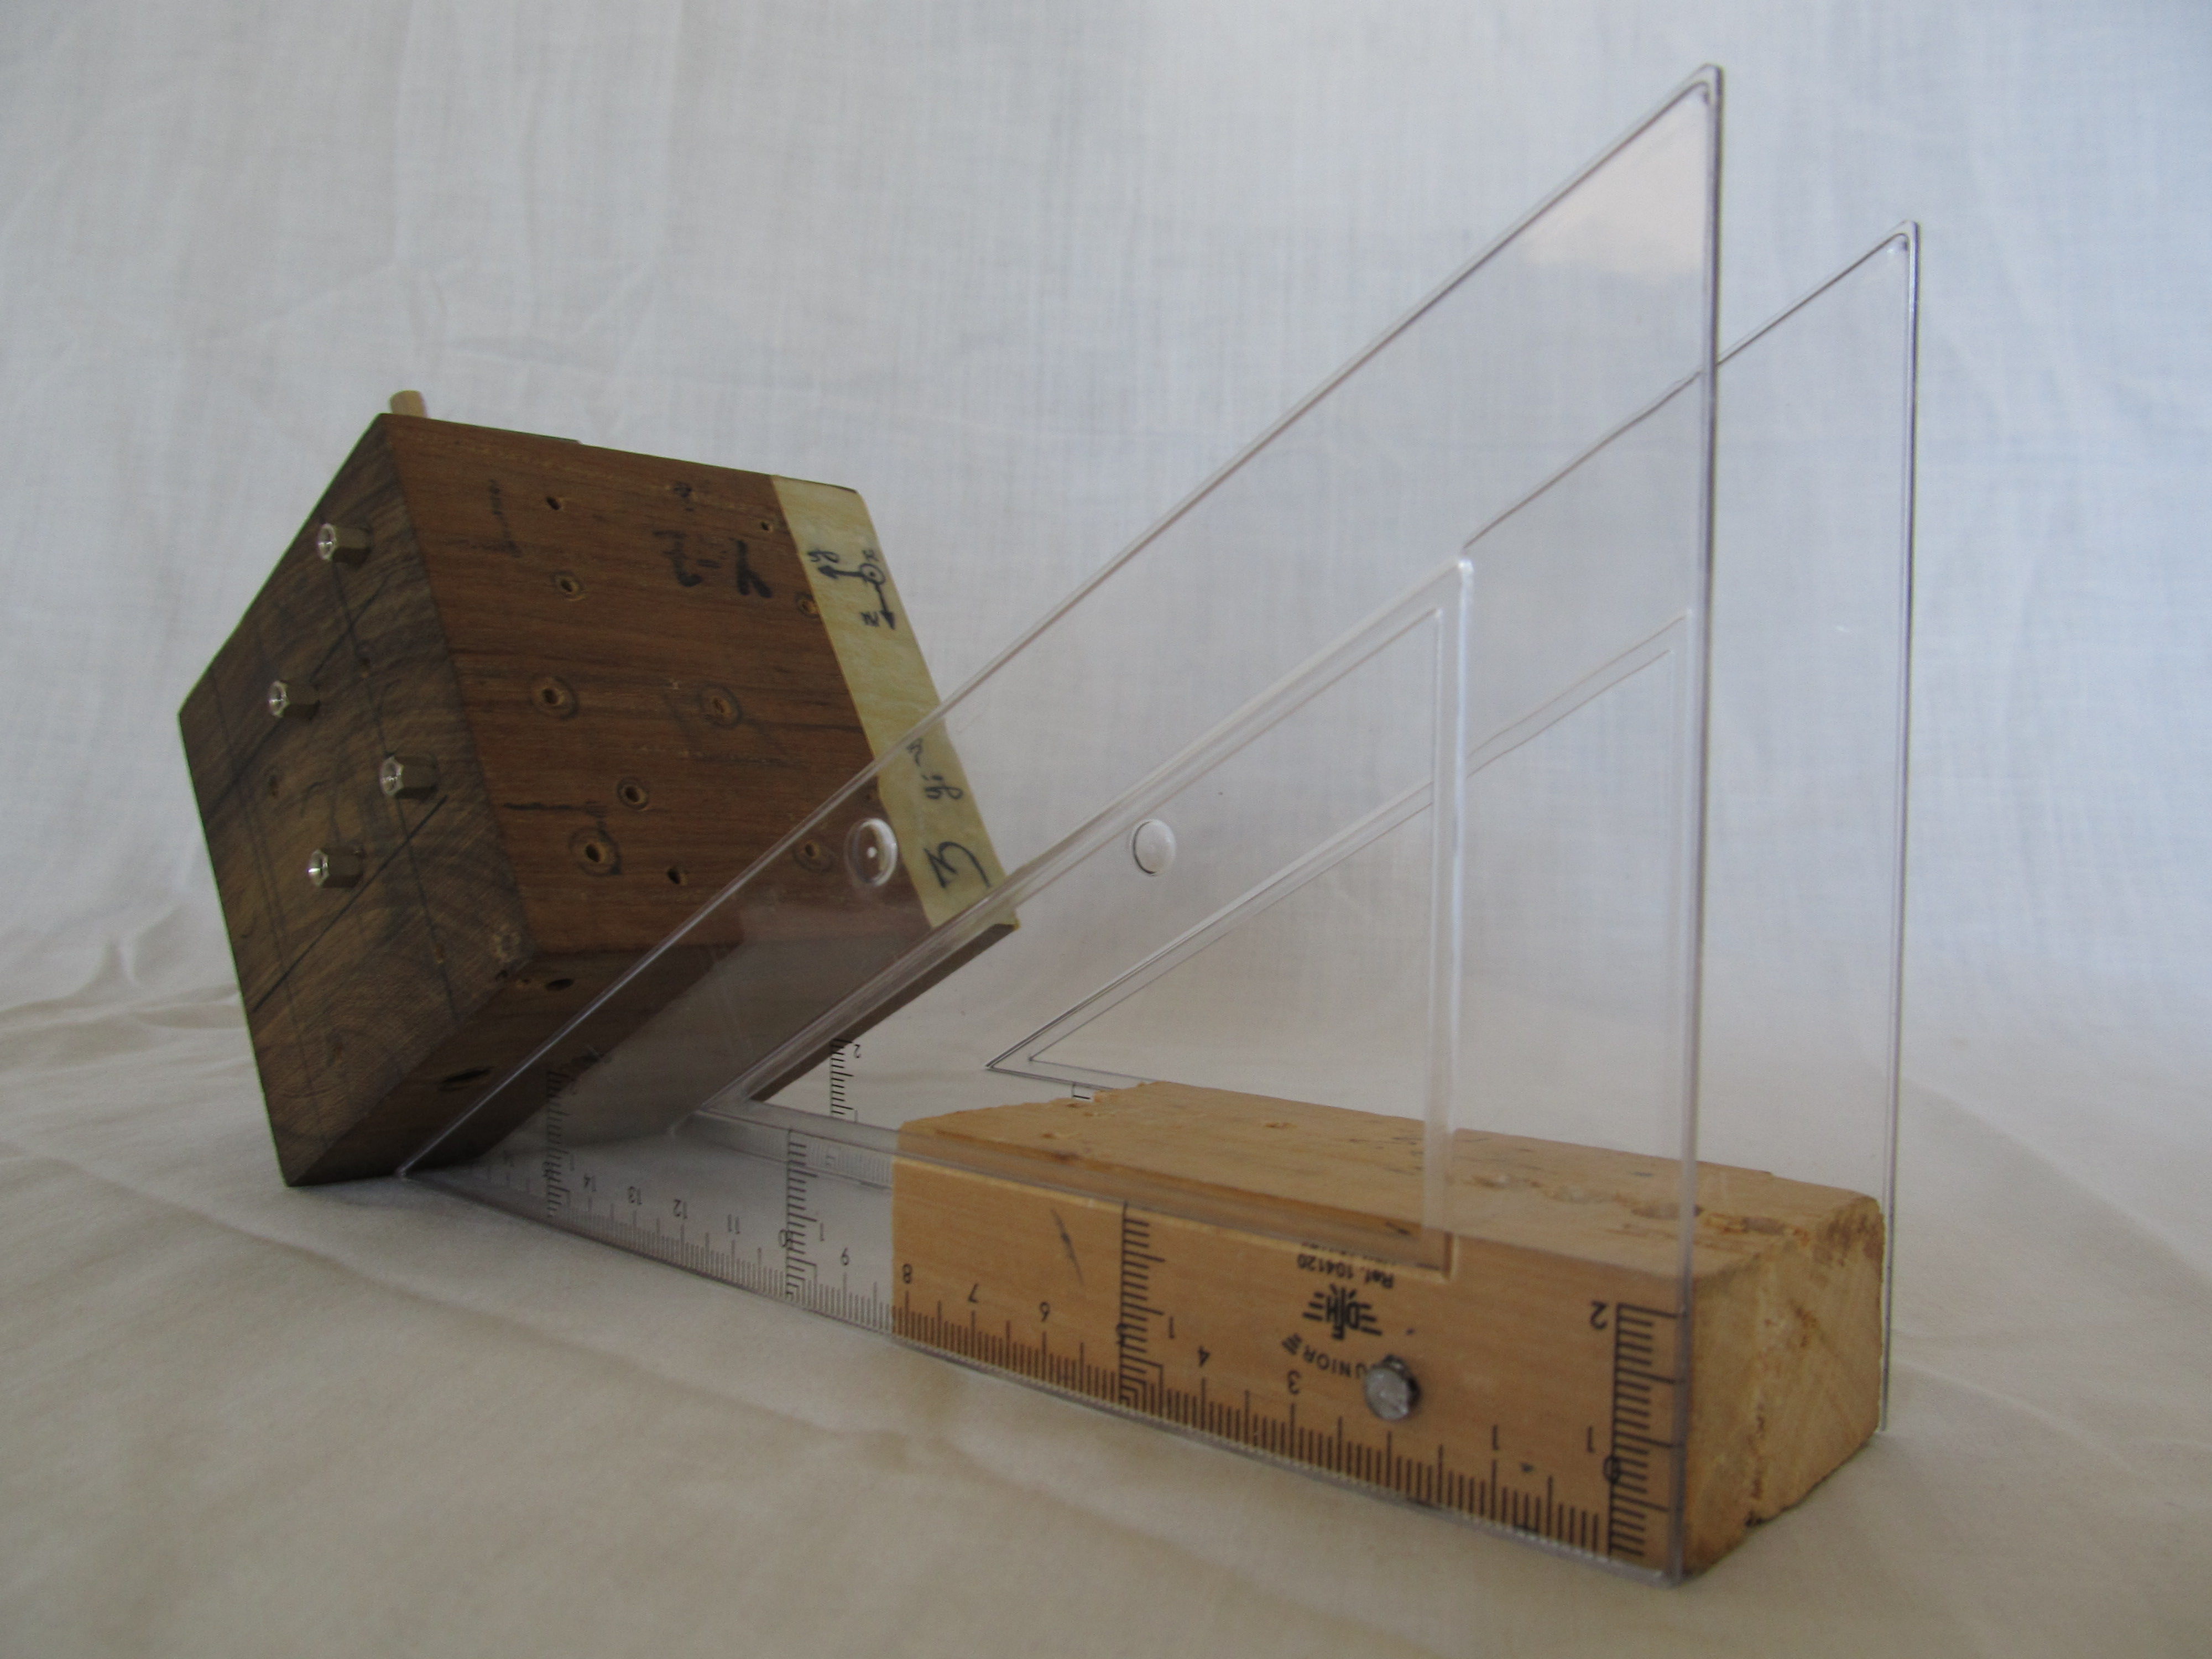
\includegraphics[width=0.45\textwidth]
    	{./pics/escuadra.jpg}
  \end{center}
  \vspace{-20pt}
  \caption{Escuadras}
  \label{fig:escuadras}
  \vspace{-10pt}
\end{wrapfigure}




















\section{Procedimiento}

\subsection{Parte I: Calibración}

\subsubsection*{Medidas a Velocidad angular constante}
En primer lugar se debe obtener la velocidad angular del tocadiscos. Se toma el tiempo que demora el tocadiscos en dar 10 vueltas completas. Se ubica el sistema exactamente en el centro del disco con el eje \textbf{z} perpendicular al mismo. Se toman medidas durante un minuto con una frecuencia de 100 muestras por segundo. Se repite el experimento una vez con el eje \textbf{y} perpendicular al disco y otra con el eje \textbf{x} perpendicular al disco. Se contrasta la velocidad angular en las 3 direcciones con la velocidad de giro del tocadiscos.

\subsection{Parte II: Definición del modelo}
A partir de las medidas obtenidas y los valores teóricos de las velocidades angulares en cada experimento realizado se propone una aproximación lineal y una cúbica. Se obtienen los parámetros de dichos modelos con el método de mínimos cuadrados.\\

Se ajusta la curva según los modelos propuestos. Se opta por el modelo que de una mejor respuesta.

\subsection{Parte III: Determinación de no idealidades}
A esta altura se intenta caracterizar las dos fuentes principales de no idealidades de los acelerómetros: El ruido y el Bias.

\subsubsection*{Ruido}
Se modela el ruido propio del giróscopo como gaussiano de media nula. Se toman medidas en reposo en los tres ejes durante 10 minutos. A partir de dichas medidas se estima la potencia del ruido. Se diseña un filtro para disminuir dicho ruido. Se grafican las aceleraciones de todos los experimentos realizados hasta el momento con el filtrado definido en este experimento. Se comparan las nuevas respuestas de los acelerómetros con las obtenidas antes del filtrado. 


\end{document}